% Latex file describing "Deleveraging" experiment results.
% Date: 2013-02-14

\documentclass[titlepage,abstract,letterpaper]{econtex}

\usepackage{handoutSetup}\usepackage{handoutShortcuts}

\usepackage{layouts,rotating,psfrag,amssymb}

\opt{JournalFormatting}{\renewcommand{\footnote}{\endnote}}

\begin{document}
\begin{center}
\Large Deleveraging 
\end{center}

The model is the extended version of the \cite{ctDiscrete} model employed in \cite{cssUSSaving}, where the only modification is to incorporate an unemployment insurance system.  (See the appendix to \cite{cssUSSaving} for details of the structure of the unemployment insurance system).

The economy consists of two groups of people, either ``patient'' or ``impatient.'' Under the same parameter values as \cite{ctDiscrete} except that the severance payment $\Severance=4$ and death rate $\PDies=0.05$, the ``patient'' group is calibrated to have time preference rate $\timeRate=0.0206$ so that their target wealth is 12, while the ``impatient'' group is calibrated to have $\timeRate=0.1061$ so that their target wealth is -2 (they are in debt, so their net worth is negative).

We consider three experiments focusing on how the saving rate evolves under different kinds of shocks.

\begin{enumerate}
\item Credit Cycle\\
We consider an experiment with a gradual increase and then an abrupt decrease of the severance payment. More concretely, before 2001, severance payment is equal to the baseline value, 4. From 2002 to 2007, severance payment gradually increases, $\Severance_{2002}=\Severance_{2001}+\eta_{\Severance},\Severance_{2003}=\Severance_{2001}+2\eta_{\Severance},...,\Severance_{2007}=\Severance_{2001}+6\eta_{\Severance}$. There is an abrupt reversal of severance payment at 2008, say, $\Severance_{2008}=\Severance_{2001}$ and remains at the baseline level from then on. 

We calibrate $\eta_{\Severance}=0.35$ so that debt level of the impatient group reaches 2.6 at 2007.
Figure 1 characterizes saving dynamics over such a credit cycle. Both groups cut their saving rate during credit boom, because higher severance payment makes people less painful when losing jobs. At 2008 when there is a sudden credit crunch, both groups increase their saving rate aggresively in order to have a higher target wealth.

\item Expansion of Growth Expectation\\
Before 2001, growth expectation is equal to the baseline value, 0. Growth expectation increases to $\eta_g$ from 2002 to 2007. Since 2008, growth expectation drops back to its original level, 0. Notice that the ``actual'' growth rate is always set to be zero, which means people are over-optimistic from 2002-2007. Given parameter values above, $\eta_g$ is calibrated to be 0.0363. 

Figure 2 characterizes saving dynamics under expansion of growth expectation, which is qualitatively similar to result of the first experiment. When people are over-optimistic about future, their saving rate is lower. When their expectaion becomes consistent with actual growth rate again, their saving rate becomes even higher in order to recover original target wealth.

\item Decrease of Unemployment Expectation\\
Before 2001, unemployment rate expectation is equal to the baseline value, 0.005. Unemployment rate expectation decreases to $0.005-\eta_{\urate}$ from 2002 to 2007. Since 2008, unemployment rate expectation increases to its original level, 0.005.  ``Actual'' unemployment rate is always set to be 0.005, which means people are over-optimistic from 2002-2007. In order to keep growth rate of labor income of employed consumers unchanged\footnote{Notice that in \cite{ctDiscrete}, it is given by $\PGro = \WGroPF/\erate$.}, we increase the growth expectation by the same amount from 2002 to 2007.  $\eta_{\urate}$ is calibrated to be 0.0038.

Figure 3 characterizes saving dynamics during the period when people underestimate unemployment rate. Clearly, when people are optimistic about future employment, they tend to cut their saving; when they realize low unemployment rate is not the truth, they suddenly increase savings and adjust their target wealth to original level.
\end{enumerate}


\begin{figure}
\caption{Saving Dynamics over Credit Cycle}
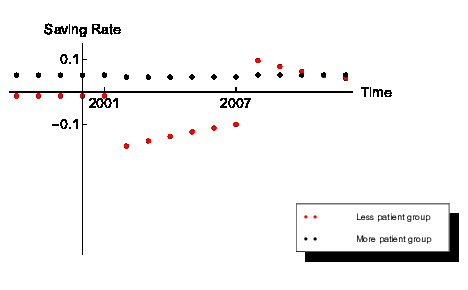
\includegraphics[width=6in]{../Figures/SavPathOverECreditCycle}

\caption{Saving Dynamics under Expansion of Growth Expectation}
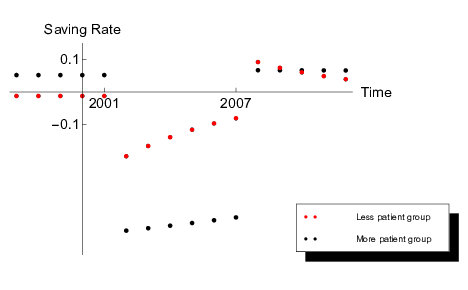
\includegraphics[width=6in]{../Figures/SavPathOverEGrowthCycle}
\end{figure}
\begin{figure}
\caption{Saving Dynamics under Optimism about Unemployment Expectation}
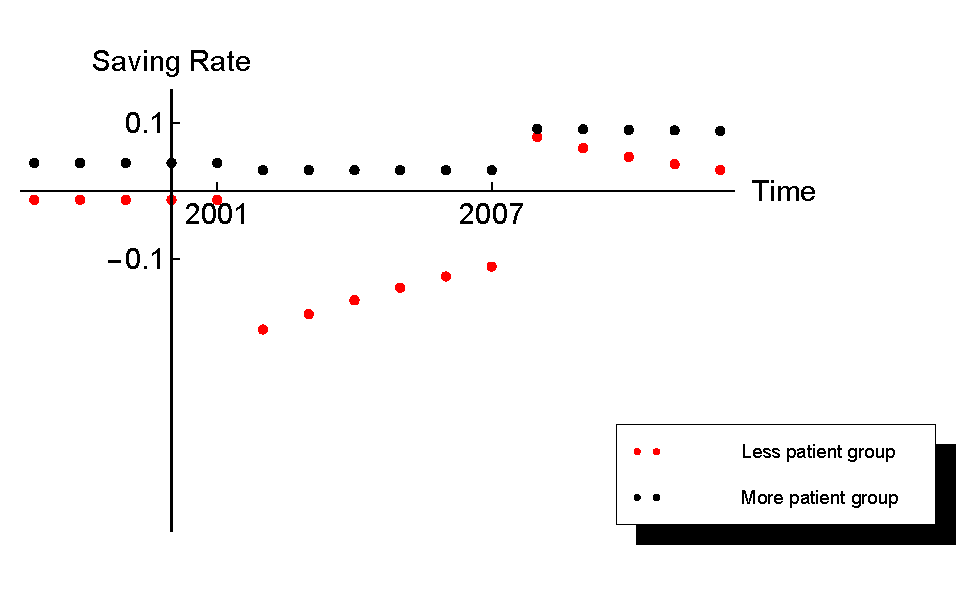
\includegraphics[width=6in]{../Figures/SavPathOverEUriskCycle}
\end{figure}

\bibliography{reference} %contains the references
\bibliographystyle{bejournal}
\end{document}

